% =====================================================================
%  Taiwanese Bankruptcy Prediction — final presentation (Augmented Decision)
%  Compile from this folder:   tectonic main.tex      (or: xelatex main.tex, twice)
%  Set in Arial (system font). Figures in figures/ are exported from the notebook by make_figures.py
% =====================================================================
\documentclass[11pt,aspectratio=169]{beamer}

% ---------- Fonts: Arial everywhere (system font) ----------
\usepackage{fontspec}
\setsansfont{Arial}
\setmonofont{Arial}
\newfontfamily\display{Arial}
\newfontfamily\light{Arial}
\usefonttheme{professionalfonts}
\hyphenpenalty=10000 \exhyphenpenalty=10000   % no hyphenation anywhere on the slides

\usepackage{amsmath, amssymb, booktabs, graphicx}
\graphicspath{{figures/}}
\usepackage{tikz, pgfplots}
\usetikzlibrary{positioning, arrows.meta, calc}
\pgfplotsset{compat=1.18}

% ---------- Palette ----------
\definecolor{paper}{HTML}{F6F3EC}
\definecolor{ink}{HTML}{16181D}
\definecolor{muted}{HTML}{6B6F78}
\definecolor{rule}{HTML}{D9D2C5}
\definecolor{risk}{HTML}{B42318}
\definecolor{model}{HTML}{155E63}
\definecolor{bench}{HTML}{B8862B}
\definecolor{risktint}{HTML}{F2DAD6}
\definecolor{modeltint}{HTML}{D5E5E3}
\definecolor{card}{HTML}{FFFEFB}

% ---------- Beamer layout ----------
\setbeamertemplate{navigation symbols}{}
\setbeamersize{text margin left=10mm, text margin right=10mm}
\setbeamercolor{background canvas}{bg=paper}
\setbeamercolor{normal text}{fg=ink}
\setbeamercolor{structure}{fg=ink}
\setbeamercolor{alerted text}{fg=risk}

\newcommand{\kicker}{}
\newcommand{\setkicker}[1]{\renewcommand{\kicker}{#1}}
\newcommand{\caps}[1]{{\ttfamily\fontsize{7.5}{9}\selectfont\addfontfeatures{LetterSpace=12}#1}}

\setbeamertemplate{frametitle}{%
  \vspace*{5.5mm}%
  {\color{risk}\caps{\kicker}}\par\vspace{1.4mm}%
  {\display\fontsize{21}{24}\selectfont\color{ink}\insertframetitle}\par\vspace{0.5mm}}

\setbeamertemplate{background}{%
  \begin{tikzpicture}
    \useasboundingbox (0,0) rectangle (\paperwidth,\paperheight);
    \fill[risk] (0,\paperheight) ++(0,-5.9mm) rectangle ++(2.4mm,-2.6mm);
  \end{tikzpicture}}

\setbeamertemplate{footline}{%
  \hspace*{10mm}{\color{muted}\caps{TAIWANESE BANKRUPTCY PREDICTION}}%
  \hfill{\color{muted}\caps{\insertframenumber\,/\,\inserttotalframenumber}}\hspace*{10mm}\par\vspace*{4.5mm}}

\setbeamertemplate{itemize item}{\raisebox{0.32ex}{\textcolor{risk}{\rule{0.7em}{1.1pt}}}}
\setbeamertemplate{enumerate item}{\textcolor{risk}{\ttfamily\bfseries\insertenumlabel}}
\newenvironment{points}{\begin{itemize}\setlength{\itemsep}{2.8mm}}{\end{itemize}}

% ---------- Building blocks ----------
\newcommand{\stat}[3][ink]{{\display\fontsize{27}{29}\selectfont\color{#1}#2}\par\vspace{1.2mm}{\footnotesize\color{muted}#3}}
\newcommand{\takeaway}[1]{{\color{risk}\rule[0.33ex]{1.3em}{1.1pt}}\;\textbf{#1}}
\newcommand{\keyformula}[2][risk]{\begin{tikzpicture}\node[fill=card, draw=#1, line width=0.6pt, rounded corners=2pt, inner xsep=4.5mm, inner ysep=2.8mm]{#2};\end{tikzpicture}}
\newcommand{\aside}[1]{{\footnotesize\color{muted}#1}}
\newcommand{\actioncard}[4][62mm]{%
  \begin{tikzpicture}
    \node[fill=card, draw=rule, rounded corners=2pt, text width=#1, inner xsep=4mm, inner ysep=2.6mm, align=left] (c)
      {{\bfseries\color{#2}#3}\\[0.4mm]{\small\color{muted}#4}};
    \fill[#2] ([yshift=-0.4mm]c.north west) rectangle ([xshift=1.3mm, yshift=0.4mm]c.south west);
  \end{tikzpicture}}
\newcommand{\step}[3]{{\color{rule}\rule{\linewidth}{0.6pt}}\par\vspace{2mm}%
  {\display\fontsize{24}{26}\selectfont\color{risk}#1}\par\vspace{2mm}{\bfseries #2}\par\vspace{1mm}{\small\color{muted}#3}}
\newcommand{\firmgrid}[2]{% 10 x 10 grid of firms; #1 = list of bankrupt cells, #2 = dot spacing
  \begin{tikzpicture}[x=#2, y=#2]
    \foreach \k in {0,...,99} {\pgfmathtruncatemacro{\i}{mod(\k,10)}\pgfmathtruncatemacro{\j}{\k/10}
      \fill[rule] (\i,-\j) circle (0.34);}
    \foreach \k in {#1} {\pgfmathtruncatemacro{\i}{mod(\k,10)}\pgfmathtruncatemacro{\j}{\k/10}
      \fill[risk] (\i,-\j) circle (0.34);}
  \end{tikzpicture}}

\newcommand{\divider}[3]{%
  {\setbeamercolor{background canvas}{bg=ink}\setbeamertemplate{background}{}%
   \begin{frame}[plain,noframenumbering]
     \begin{tikzpicture}[remember picture, overlay]
       \node[anchor=south east, inner sep=0] at ([xshift=-10mm, yshift=8mm]current page.south east)
         {\display\fontsize{130}{130}\selectfont\color{risk}#1};
       \node[anchor=north west, inner sep=0, text width=128mm, align=left] at ([xshift=10mm, yshift=-16mm]current page.north west)
         {{\color{paper!55!ink}\caps{PART #1}}\\[5mm]
          {\display\fontsize{31}{35}\selectfont\color{paper}#2}\\[5mm]
          {\light\large\color{paper!72!ink}#3}};
     \end{tikzpicture}
   \end{frame}}}

\begin{document}

% =====================================================================
%  TITLE
% =====================================================================
{\setbeamertemplate{background}{}
\begin{frame}[plain]
  \begin{tikzpicture}[remember picture, overlay]
    \fill[risk] ([yshift=-14mm]current page.north west) rectangle ++(2.4mm,-2.6mm);
    \node[anchor=north west, inner sep=0, text width=96mm, align=left] at ([xshift=10mm, yshift=-13.6mm]current page.north west)
      {{\color{risk}\caps{AUGMENTED DECISION \quad·\quad FINAL PROJECT}}\\[6mm]
       {\display\fontsize{28}{33}\selectfont Flagging bankruptcy\\ \textit{before} it happens}\\[5mm]
       {\light\large\color{muted} Cost-sensitive screening of Taiwanese firms\\ with LASSO selection and a decision tree}};
    \node[anchor=south west, inner sep=0, text width=140mm, align=left] at ([xshift=10mm, yshift=8mm]current page.south west)
      {{\color{rule}\rule{140mm}{0.6pt}}\\[3mm]
       {\small\bfseries Yassine ERRAJI \enspace·\enspace William PELTIER \enspace·\enspace Ben DAESH \enspace·\enspace Simon AMAR}\\[1.5mm]
       {\color{muted}\caps{23 OCTOBER 2026}}};
    \node[anchor=north east, inner sep=0] at ([xshift=-13mm, yshift=-16mm]current page.north east) {\firmgrid{17,54,88}{3.8mm}};
    \node[anchor=north east, inner sep=0, align=right] at ([xshift=-12mm, yshift=-55mm]current page.north east)
      {\color{muted}\caps{100 FIRMS \quad·\quad 3 GO BANKRUPT}};
  \end{tikzpicture}
\end{frame}}

% =====================================================================
%  OPENING
% =====================================================================
\setkicker{THE QUESTION}
\begin{frame}{Should this firm be flagged?}
  \vspace{5mm}
  \begin{columns}[T,onlytextwidth]
    \column{0.52\textwidth}
      A credit analyst reads a listed firm's financial ratios and must choose one of two actions:\par\vspace{4mm}
      \actioncard{risk}{Flag}{deny or reprice credit, open a closer review}\par\vspace{2.5mm}
      \actioncard{model}{Do not flag}{business as usual}
    \column{0.40\textwidth}
      \vspace{1mm}
      {\display\Large Our goal}\par\vspace{3mm}
      A decision rule that is \textbf{cheap on average}\ldots\par\vspace{2mm}
      \ldots and that the analyst can \textbf{read and question}.
  \end{columns}
\end{frame}

\setkicker{ROADMAP}
\begin{frame}{Four steps}
  \vspace{8mm}
  \begin{columns}[T,onlytextwidth]
    \column{0.22\textwidth}\step{01}{Problem formulation}{Costs, metric and a first look at the data}
    \column{0.22\textwidth}\step{02}{Variable selection}{LASSO keeps 43 of the 94 ratios}
    \column{0.22\textwidth}\step{03}{Model selection}{Tune the tree, compare candidates}
    \column{0.22\textwidth}\step{04}{Evaluation}{One look at 1,364 unseen firms}
  \end{columns}
\end{frame}

% =====================================================================
%  01 PROBLEM FORMULATION
% =====================================================================
\divider{01}{Problem formulation}{What are we predicting, and how do we score a decision?}
\setkicker{01 \quad·\quad PROBLEM FORMULATION}

\begin{frame}{The data}
  \vspace{9mm}
  \begin{columns}[T,onlytextwidth]
    \column{0.22\textwidth}\stat{6,819}{listed Taiwanese firms}
    \column{0.17\textwidth}\stat{95}{financial ratios per firm}
    \column{0.30\textwidth}\stat{11 years}{1999–2009, Taiwan Economic Journal}
    \column{0.24\textwidth}\stat[risk]{3.2\,\%}{went bankrupt (220 firms)}
  \end{columns}
  \vfill
  \aside{Source: UCI Machine Learning Repository, \emph{Taiwanese Bankruptcy Prediction}, doi:10.24432/C5004D.}
  \vspace{3mm}
\end{frame}

\begin{frame}{Accuracy is a trap}
  \vspace{3mm}
  \begin{columns}[c,onlytextwidth]
    \column{0.40\textwidth}\centering
      \firmgrid{97,98,99}{4.4mm}\par\vspace{2mm}
      {\color{muted}\caps{1 DOT = 68 FIRMS}}
    \column{0.55\textwidth}
      A model that \textbf{never flags anyone} is\par\vspace{1mm}
      {\display\fontsize{30}{32}\selectfont 96.8\,\%}\;{\display\Large\color{muted}accurate}\par\vspace{2mm}
      \ldots and catches {\color{risk}\bfseries 0 bankruptcies}.\par\vspace{6mm}
      \takeaway{We need a metric that knows a missed bankruptcy is worse than a false alarm.}
  \end{columns}
\end{frame}

\begin{frame}{Mistakes do not cost the same}
  \vspace{3mm}\centering
  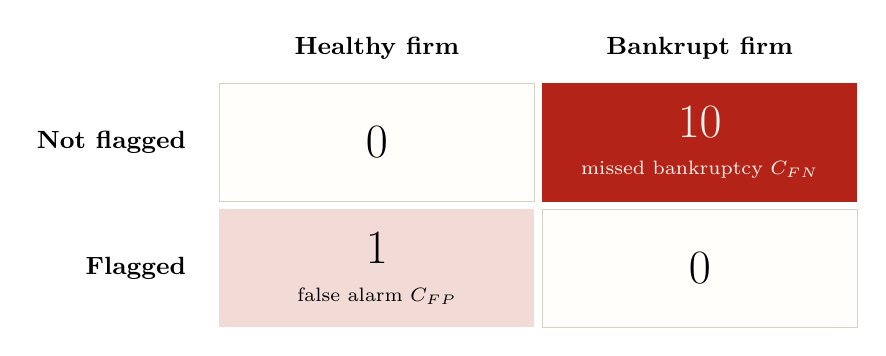
\begin{tikzpicture}[x=1mm, y=1mm, cell/.style={minimum width=40mm, minimum height=15mm, align=center, inner sep=0},
                      head/.style={font=\small\bfseries}]
    \node[head] at (45,12) {Healthy firm};
    \node[head] at (86,12) {Bankrupt firm};
    \node[head, anchor=east] at (22,0) {Not flagged};
    \node[head, anchor=east] at (22,-16) {Flagged};
    \node[cell, fill=card, draw=rule] at (45,0) {\display\LARGE 0};
    \node[cell, fill=risk, text=paper] at (86,0) {{\display\LARGE 10}\\[0.6mm]{\scriptsize missed bankruptcy $C_{FN}$}};
    \node[cell, fill=risktint] at (45,-16) {{\display\LARGE 1}\\[0.6mm]{\scriptsize false alarm $C_{FP}$}};
    \node[cell, fill=card, draw=rule] at (86,-16) {\display\LARGE 0};
  \end{tikzpicture}\par\vspace{6mm}
  \raggedright
  \takeaway{A missed bankruptcy is assumed to cost as much as 10 false alarms.}\par\vspace{1mm}
  \aside{Stipulated, not estimated: Step 4 tests cost ratios of 5 and 20.}
\end{frame}

\begin{frame}{From costs to a decision rule}
  \vspace{2mm}
  \begin{columns}[c,onlytextwidth]
    \column{0.47\textwidth}
      For a firm with bankruptcy probability $p = P(Y=1 \mid x)$:\par\vspace{3mm}
      \begin{tabular}{@{}ll@{}}
        expected cost if we \textbf{flag}: & $C_{FP}\,(1-p)$\\[1.5mm]
        expected cost if we \textbf{do not}: & $C_{FN}\,p$
      \end{tabular}\par\vspace{4mm}
      Flag when flagging is cheaper:\par\vspace{2mm}
      \keyformula{$\displaystyle p \;\ge\; \frac{C_{FP}}{C_{FP}+C_{FN}} \;=\; \frac{1}{11} \;\approx\; 0.09$}\par\vspace{1.5mm}
      \aside{Bayes decision rule (Lecture 1).}
    \column{0.48\textwidth}
      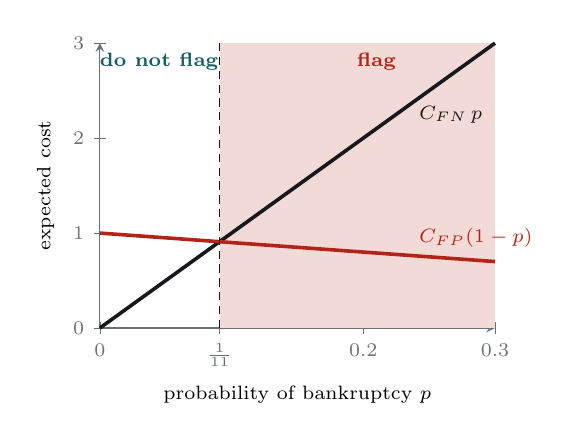
\begin{tikzpicture}
        \begin{axis}[width=66mm, height=52mm, xmin=0, xmax=0.3, ymin=0, ymax=3, axis lines=left,
                     axis line style={muted}, tick style={muted}, tick label style={font=\scriptsize, color=muted},
                     label style={font=\scriptsize}, xlabel={probability of bankruptcy $p$}, ylabel={expected cost},
                     xtick={0, 0.0909, 0.2, 0.3}, xticklabels={0, $\frac{1}{11}$, 0.2, 0.3}, ytick={0,1,2,3},
                     every axis plot/.append style={line width=1.3pt}, clip=false]
          \fill[risktint] (axis cs:0.0909,0) rectangle (axis cs:0.3,3);
          \node[font=\scriptsize\bfseries, text=risk] at (axis cs:0.21,2.8) {flag};
          \node[font=\scriptsize\bfseries, text=model] at (axis cs:0.045,2.8) {do not flag};
          \addplot[ink, domain=0:0.3, samples=2] {10*x};
          \addplot[risk, domain=0:0.3, samples=2] {1-x};
          \draw[ink, densely dashed, thin] (axis cs:0.0909,0) -- (axis cs:0.0909,3);
          \node[font=\scriptsize, text=ink, anchor=west] at (axis cs:0.235,2.25) {$C_{FN}\,p$};
          \node[font=\scriptsize, text=risk, anchor=west] at (axis cs:0.235,0.95) {$C_{FP}(1-p)$};
        \end{axis}
      \end{tikzpicture}
  \end{columns}
\end{frame}

\begin{frame}{How we score a model}
  \vspace{4mm}
  \begin{columns}[c,onlytextwidth]
    \column{0.56\textwidth}
      The \textbf{average cost per firm}: the empirical risk under the loss table.\par\vspace{4mm}
      \keyformula{$\displaystyle \hat R_n \;=\; \frac{1}{n}\sum_{i=1}^{n} L(\hat a_i, y_i) \;=\; \frac{10\cdot \text{FN} + 1\cdot\text{FP}}{n}$}\par\vspace{3mm}
      \aside{Lower is better. Recall and precision are reported alongside it.}
    \column{0.36\textwidth}
      \stat[muted]{0.32}{cost of ``never flag'' \;($10 \times 3.2\,\%$)}\par\vspace{4mm}
      \takeaway{The bar every model must clear.}
  \end{columns}
\end{frame}

\begin{frame}{Many ratios say the same thing}
  \vspace{1mm}
  \begin{columns}[c,onlytextwidth]
    \column{0.52\textwidth}\centering
      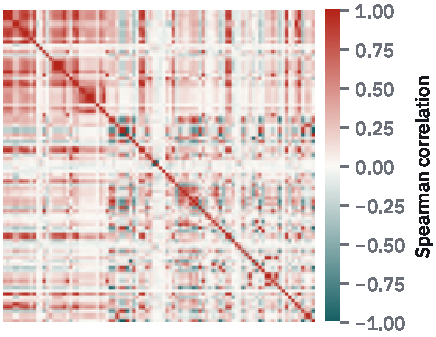
\includegraphics{heatmap.pdf}
    \column{0.44\textwidth}
      \stat[risk]{50 pairs}{of ratios with $|\rho| > 0.95$, involving 47 of the 94 ratios}\par\vspace{5mm}
      \aside{Spearman correlation: it captures a ratio and its inverse, and ignores extreme magnitudes.}\par\vspace{5mm}
      \takeaway{A strong case for variable selection.}
  \end{columns}
\end{frame}

\begin{frame}{Some values are off the scale}
  \vspace{5mm}\centering
  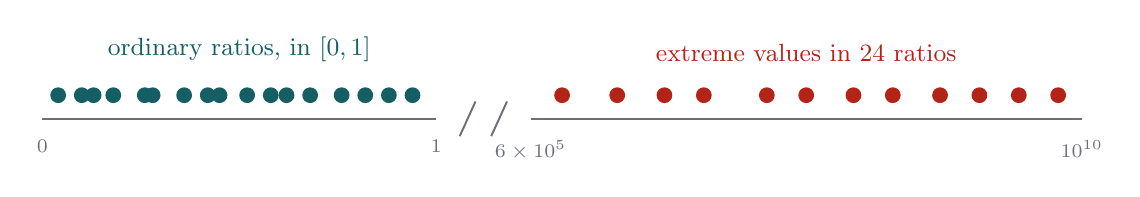
\begin{tikzpicture}[x=1mm, y=1mm]
    \draw[muted, line width=0.7pt] (0,0) -- (50,0);
    \draw[muted, line width=0.7pt] (62,0) -- (132,0);
    \draw[muted, line width=0.7pt] (53,-2.2) -- (55,2.2);
    \draw[muted, line width=0.7pt] (57,-2.2) -- (59,2.2);
    \foreach \x/\l in {0/0, 50/1, 62/{$6 \times 10^{5}$}, 132/{$10^{10}$}} \node[below=1.5mm, font=\scriptsize, text=muted] at (\x,0) {\l};
    \foreach \x in {2,5,6.5,9,13,14,18,21,22.5,26,29,31,34,38,41,44,47} \fill[model] (\x,3) circle (1);
    \foreach \x in {66,73,79,84,92,97,103,108,114,119,124,129} \fill[risk] (\x,3) circle (1);
    \node[font=\small, text=model, above] at (25,6) {ordinary ratios, in $[0,1]$};
    \node[font=\small, text=risk, above] at (97,6) {extreme values in 24 ratios};
  \end{tikzpicture}\par\vspace{9mm}\raggedright
  \begin{points}
    \item \textbf{Not noise:} inside the extreme group, the value alone still ranks bankruptcies with an AUC of 0.72.
    \item \textbf{Our answer:} keep the \emph{order}, drop the magnitude. The tree only uses order; the LASSO gets a rank (quantile) transform.
  \end{points}
\end{frame}

\begin{frame}{Our approach in one picture}
  \vspace{8mm}\centering
  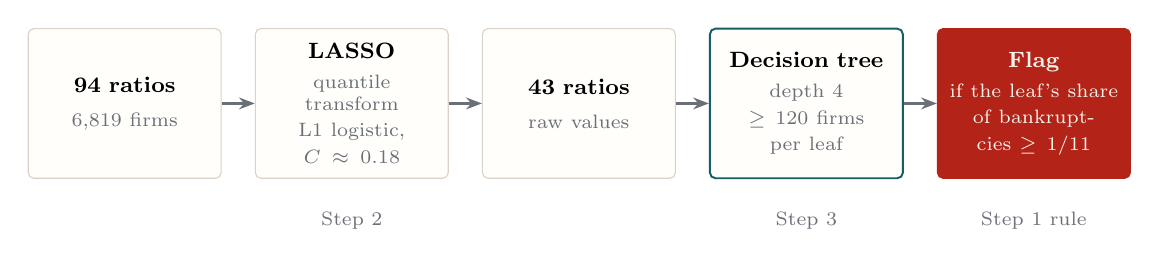
\begin{tikzpicture}[node distance=4.2mm, box/.style={draw=rule, fill=card, rounded corners=2pt, align=center, text width=21.5mm,
                      minimum height=19mm, inner sep=1.5mm, font=\footnotesize}, arr/.style={-{Stealth[length=2mm]}, muted, line width=0.8pt}]
    \node[box] (a) {\textbf{94 ratios}\\[1mm]{\scriptsize\color{muted}6,819 firms}};
    \node[box, right=of a] (b) {\textbf{LASSO}\\[1mm]{\scriptsize\color{muted}quantile transform\\L1 logistic, $C \approx 0.18$}};
    \node[box, right=of b] (c) {\textbf{43 ratios}\\[1mm]{\scriptsize\color{muted}raw values}};
    \node[box, right=of c, draw=model, line width=0.7pt] (d) {\textbf{Decision tree}\\[1mm]{\scriptsize\color{muted}depth 4\\$\ge 120$ firms per leaf}};
    \node[box, right=of d, fill=risk, draw=risk, text=paper] (e) {\textbf{Flag}\\[1mm]{\scriptsize if the leaf's share\\of bankruptcies $\ge 1/11$}};
    \foreach \u/\v in {a/b, b/c, c/d, d/e} \draw[arr] (\u) -- (\v);
    \node[below=3mm of b, font=\scriptsize, text=muted] {Step 2};
    \node[below=3mm of d, font=\scriptsize, text=muted] {Step 3};
    \node[below=3mm of e, font=\scriptsize, text=muted] {Step 1 rule};
  \end{tikzpicture}\par\vspace{10mm}\raggedright
  \takeaway{Everything is fitted on the training set. The test set is opened once.}
\end{frame}

% =====================================================================
%  02 VARIABLE SELECTION
% =====================================================================
\divider{02}{Variable selection}{Which of the 94 ratios do we really need?}
\setkicker{02 \quad·\quad VARIABLE SELECTION}

\begin{frame}{LASSO for a yes/no outcome}
  \vspace{1mm}\centering
  \keyformula{$\displaystyle \min_{b_0,\,\beta}\;\; \underbrace{-\frac{1}{n}\sum_{i=1}^{n}\Big[y_i\log p_i + (1-y_i)\log(1-p_i)\Big]}_{\text{fit to the data}} \;+\; \underbrace{\lambda\,\lVert\beta\rVert_1}_{\text{L1 penalty}}$}\par\vspace{3mm}
  \raggedright
  \begin{points}
    \item The L1 penalty sets many coefficients to \textbf{exactly zero}: those ratios are dropped (Lecture 4).
    \item \textbf{One knob}, $\lambda$ (or $C = 1/n\lambda$), sets how many ratios survive.
    \item Fast enough to be \textbf{refit inside every cross-validation fold}.
  \end{points}
\end{frame}

\begin{frame}{Choosing the penalty}
  \vspace{2mm}\centering
  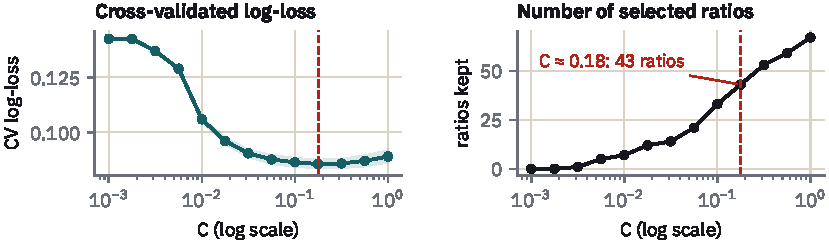
\includegraphics{lasso_path.pdf}\par\vspace{4mm}\raggedright
  \takeaway{Lowest cross-validated log-loss at $C \approx 0.18$: 43 of the 94 ratios are kept.}
\end{frame}

\begin{frame}{Is the shortlist stable?}
  \vspace{2mm}\centering
  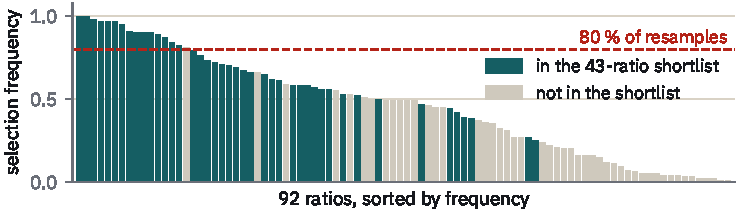
\includegraphics{stability.pdf}\par\vspace{3mm}\raggedright
  \aside{100 bootstrap refits of the whole procedure. Only 15 of the 43 ratios survive at least 80\,\% of the time.}\par\vspace{2mm}
  \takeaway{Correlated ratios swap places: a predictive shortlist, not a list of causes.}
\end{frame}

% =====================================================================
%  03 MODEL SELECTION
% =====================================================================
\divider{03}{Model selection \& tuning}{How deep should the tree grow, and does selection really help?}
\setkicker{03 \quad·\quad MODEL SELECTION}

\begin{frame}{How a tree flags a firm}
  \vspace{4mm}
  \begin{columns}[c,onlytextwidth]
    \column{0.47\textwidth}\centering
      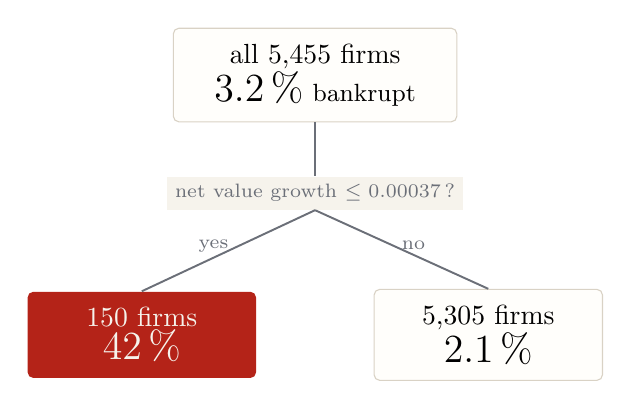
\begin{tikzpicture}[x=1mm, y=1mm, box/.style={align=center, rounded corners=2pt, inner sep=2mm, text width=25mm}]
        \node[box, draw=rule, fill=card, text width=32mm] (r) at (30,0) {all 5,455 firms\\{\display\Large 3.2\,\%} \small bankrupt};
        \node[font=\scriptsize, text=muted, fill=paper, inner sep=1mm] (q) at (30,-15) {net value growth $\le 0.00037$\,?};
        \node[box, fill=risk, text=paper] (l) at (8,-33) {150 firms\\{\display\Large 42\,\%}};
        \node[box, draw=rule, fill=card] (rr) at (52,-33) {5,305 firms\\{\display\Large 2.1\,\%}};
        \draw[muted, line width=0.7pt] (r.south) -- (q.north);
        \draw[muted, line width=0.7pt] (q.south) -- (l.north) node[pos=0.45, left=1mm, font=\scriptsize, text=muted, inner sep=0] {yes};
        \draw[muted, line width=0.7pt] (q.south) -- (rr.north) node[pos=0.45, right=1mm, font=\scriptsize, text=muted, inner sep=0] {no};
      \end{tikzpicture}
    \column{0.47\textwidth}
      Splits make the leaves \textbf{purer}, measured by the Gini impurity:\par\vspace{2mm}
      \keyformula[model]{$G(q) = 2q(1-q)$}\par\vspace{3mm}
      Each leaf's \textbf{share of bankruptcies} $\hat\eta(x)$ estimates $P(Y=1 \mid x)$.\par\vspace{2mm}
      \takeaway{Flag the firm if $\hat\eta(x) \ge 1/11$.}
  \end{columns}
\end{frame}

\begin{frame}{An honest protocol}
  \vspace{6mm}\centering
  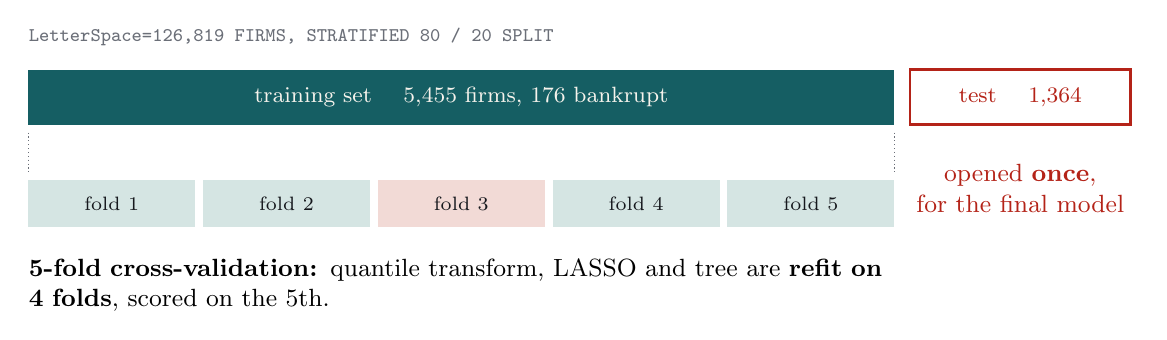
\begin{tikzpicture}[x=1mm, y=1mm]
    \node[anchor=south west, inner sep=0, text=muted] at (0,30) {\caps{6,819 FIRMS, STRATIFIED 80 / 20 SPLIT}};
    \fill[model] (0,20) rectangle (110,27);
    \node[text=paper, font=\footnotesize] at (55,23.5) {training set \quad 5,455 firms, 176 bankrupt};
    \draw[risk, line width=0.9pt] (112,20) rectangle (140,27);
    \node[text=risk, font=\footnotesize] at (126,23.5) {test \quad 1,364};
    \foreach \i in {0,...,4} \fill[modeltint] (\i*22.2,7) rectangle ++(21.2,6);
    \fill[risktint] (2*22.2,7) rectangle ++(21.2,6);
    \foreach \i in {0,...,4} \node[font=\scriptsize, text=ink] at (\i*22.2+10.6,10) {fold \pgfmathparse{int(\i+1)}\pgfmathresult};
    \draw[muted, densely dotted] (0,19) -- (0,14); \draw[muted, densely dotted] (110,19) -- (110,14);
    \node[anchor=north west, font=\small, text width=110mm, align=left, inner sep=0] at (0,3)
      {\textbf{5-fold cross-validation:} quantile transform, LASSO and tree are \textbf{refit on 4 folds}, scored on the 5th.};
    \node[anchor=north, font=\small, text=risk, text width=30mm, align=center, inner sep=0] at (126,15)
      {opened \textbf{once},\\for the final model};
  \end{tikzpicture}\par\vspace{7mm}\raggedright
  \takeaway{No decision ever sees the test set.}
\end{frame}

\begin{frame}{Leaves must be large}
  \vspace{2mm}\centering
  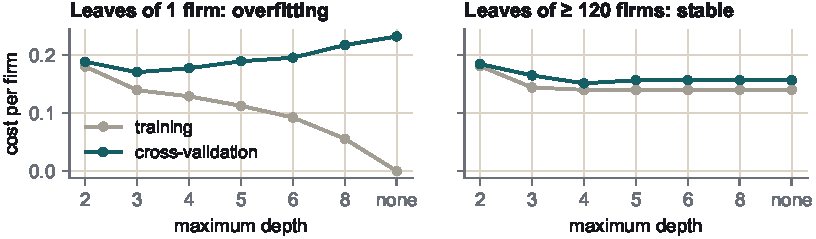
\includegraphics{validation.pdf}\par\vspace{2mm}\raggedright
  \aside{Leaves of one firm memorise the data: training cost falls to 0, CV cost climbs to 0.23.}\par\vspace{1.5mm}
  \takeaway{With at least 120 firms per leaf, depth 4 is best: 0.151 per firm.}
\end{frame}

\begin{frame}{Four candidates, same five folds}
  \vspace{3mm}\centering
  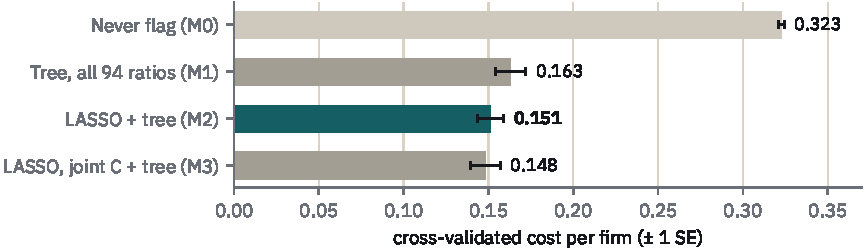
\includegraphics{candidates.pdf}\par\vspace{4mm}\raggedright
  \takeaway{Every tree halves the cost of never flagging.}
\end{frame}

\begin{frame}{Does selection really help?}
  \vspace{2mm}
  \begin{columns}[c,onlytextwidth]
    \column{0.60\textwidth}
      Same folds, so we compare \textbf{fold by fold}:\par\vspace{2mm}
      \keyformula{$\displaystyle \bar\Delta \pm \frac{s_\Delta}{\sqrt{5}}, \qquad \Delta_k = \text{cost}_k(\text{M2}) - \text{cost}_k(\text{other})$}\par\vspace{4mm}
      {\small
      \begin{tabular}{@{}lrl@{}}
        \toprule
        vs M2 & gain & verdict \\
        \midrule
        M1, all 94 ratios & $-0.012 \pm 0.005$ & never beats M2 \\
        M3, joint $C$ (7 ratios) & $+0.003 \pm 0.007$ & within noise \\
        \bottomrule
      \end{tabular}}\par\vspace{4mm}
      \takeaway{Selection helps. We keep M2.}
    \column{0.36\textwidth}\centering
      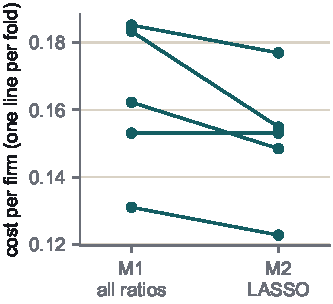
\includegraphics[width=\linewidth]{paired.pdf}
  \end{columns}
\end{frame}

\begin{frame}{The price of interpretability}
  \vspace{2mm}
  \begin{columns}[T,onlytextwidth]
    \column{0.46\textwidth}
      {\color{model}\caps{OUR CHOICE}}\par\vspace{1mm}
      {\display\Large One decision tree (M2)}\par\vspace{2.5mm}
      \stat[model]{0.151}{cross-validated cost per firm}\par\vspace{2.5mm}
      9 leaves, 8 ratios: \textbf{every decision is a readable rule.}
    \column{0.46\textwidth}
      {\color{bench}\caps{BENCHMARK ONLY}}\par\vspace{1mm}
      {\display\Large A random forest (M4)}\par\vspace{2.5mm}
      \stat[bench]{0.136}{cross-validated cost per firm}\par\vspace{2.5mm}
      300 trees vote: finer probabilities, \textbf{but no rule to read.}
  \end{columns}
  \vfill
  \takeaway{The forest saves about 10\,\% ($0.015 \pm 0.007$): the price of readable rules.}
  \vspace{2mm}
\end{frame}

% =====================================================================
%  04 EVALUATION
% =====================================================================
\divider{04}{Evaluation}{One look at 1,364 firms the model has never seen.}
\setkicker{04 \quad·\quad EVALUATION}

\begin{frame}{The final tree}
  \vspace{1mm}\centering
  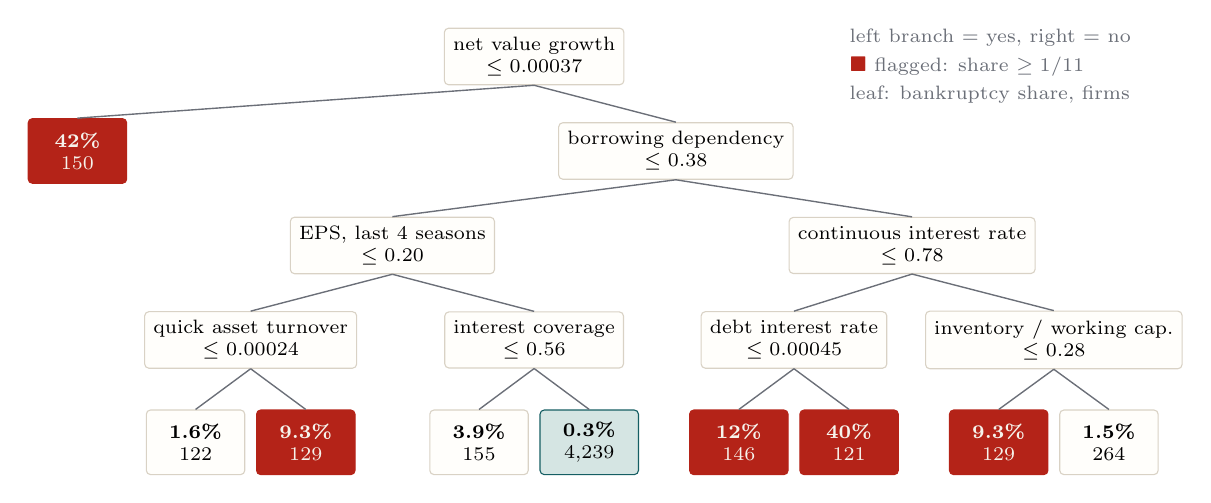
\begin{tikzpicture}[x=1mm, y=1mm, font=\scriptsize,
      split/.style={draw=rule, fill=card, rounded corners=1.5pt, align=center, inner sep=1.1mm},
      leaf/.style={draw=rule, fill=card, rounded corners=1.5pt, align=center, inner sep=0.8mm, minimum width=12.5mm, minimum height=8.2mm},
      flag/.style={leaf, fill=risk, draw=risk, text=paper},
      e/.style={draw=muted, line width=0.5pt}]
    \node[split] (n0)  at (70,0)    {net value growth\\$\le 0.00037$};
    \node[flag]  (n1)  at (12,-12)  {\textbf{42\%}\\150};
    \node[split] (n2)  at (88,-12)  {borrowing dependency\\$\le 0.38$};
    \node[split] (n3)  at (52,-24)  {EPS, last 4 seasons\\$\le 0.20$};
    \node[split] (n10) at (118,-24) {continuous interest rate\\$\le 0.78$};
    \node[split] (n4)  at (34,-36)  {quick asset turnover\\$\le 0.00024$};
    \node[split] (n7)  at (70,-36)  {interest coverage\\$\le 0.56$};
    \node[split] (n11) at (103,-36) {debt interest rate\\$\le 0.00045$};
    \node[split] (n14) at (136,-36) {inventory / working cap.\\$\le 0.28$};
    \node[leaf]  (n5)  at (27,-49)  {\textbf{1.6\%}\\122};
    \node[flag]  (n6)  at (41,-49)  {\textbf{9.3\%}\\129};
    \node[leaf]  (n8)  at (63,-49)  {\textbf{3.9\%}\\155};
    \node[leaf, fill=modeltint, draw=model] (n9) at (77,-49) {\textbf{0.3\%}\\4,239};
    \node[flag]  (n12) at (96,-49)  {\textbf{12\%}\\146};
    \node[flag]  (n13) at (110,-49) {\textbf{40\%}\\121};
    \node[flag]  (n15) at (129,-49) {\textbf{9.3\%}\\129};
    \node[leaf]  (n16) at (143,-49) {\textbf{1.5\%}\\264};
    \foreach \a/\b in {n0/n1, n0/n2, n2/n3, n2/n10, n3/n4, n3/n7, n10/n11, n10/n14, n4/n5, n4/n6, n7/n8, n7/n9, n11/n12, n11/n13, n14/n15, n14/n16}
      \draw[e] (\a.south) -- (\b.north);
    \node[anchor=north west, align=left, text=muted, inner sep=0] at (110,3.5)
      {left branch = yes, right = no\\[0.8mm]
       {\color{risk}$\blacksquare$} flagged: share $\ge 1/11$\\[0.8mm]
       leaf: bankruptcy share, firms};
  \end{tikzpicture}
\end{frame}

\begin{frame}{Reading the tree}
  \vspace{3mm}
  \begin{columns}[T,onlytextwidth]
    \column{0.56\textwidth}
      {\color{risk}\caps{THREE ALARMS}}\par\vspace{2mm}
      \begin{enumerate}\setlength{\itemsep}{2.6mm}
        \item \textbf{Weakest net value growth} (bottom 2.7\,\%): 42\,\% go bankrupt.
        \item \textbf{Heavy borrowing + weak profitability}: 40\,\% when the debt is expensive, 12\,\% otherwise.
        \item \textbf{Two narrower pockets} at 9.3\,\%: flagged, but only just.
      \end{enumerate}
    \column{0.38\textwidth}
      {\color{model}\caps{ONE SAFE ZONE}}\par\vspace{2mm}
      Moderate borrowing, EPS above 0.20, interest coverage above 0.56:\par\vspace{3mm}
      \stat[model]{0.3\,\%}{bankrupt, in a leaf holding 78\,\% of the firms}\par\vspace{5mm}
      \aside{Predictive associations, not causal effects.}
  \end{columns}
\end{frame}

\begin{frame}{Results on unseen firms}
  \vspace{3mm}
  \begin{columns}[c,onlytextwidth]
    \column{0.50\textwidth}
      \stat[model]{0.179 \;{\color{muted}\fontsize{15}{17}\selectfont vs 0.323}}{cost per firm, model vs never flag: \textbf{$-$45\,\%}}\par\vspace{5mm}
      \begin{columns}[T,onlytextwidth]
        \column{0.5\linewidth}\stat{32 / 44}{bankruptcies caught}
        \column{0.5\linewidth}\stat{156}{firms flagged (1 in 9)}
      \end{columns}
    \column{0.44\textwidth}\centering
      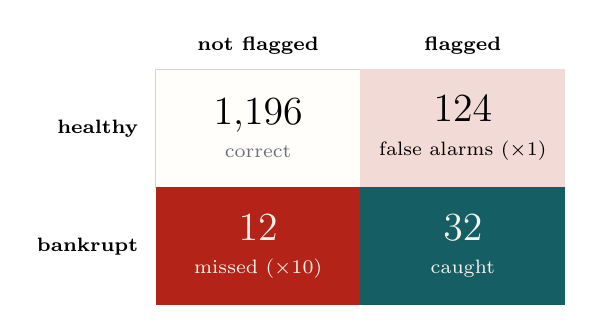
\begin{tikzpicture}[x=1mm, y=1mm, cell/.style={minimum width=26mm, minimum height=15mm, align=center, inner sep=0}]
        \node[font=\scriptsize\bfseries] at (13,10.5) {not flagged};
        \node[font=\scriptsize\bfseries] at (39,10.5) {flagged};
        \node[font=\scriptsize\bfseries, anchor=east] at (-1,0) {healthy};
        \node[font=\scriptsize\bfseries, anchor=east] at (-1,-15) {bankrupt};
        \node[cell, fill=card, draw=rule] at (13,0) {{\display\Large 1,196}\\{\scriptsize\color{muted}correct}};
        \node[cell, fill=risktint] at (39,0) {{\display\Large 124}\\{\scriptsize false alarms ($\times 1$)}};
        \node[cell, fill=risk, text=paper] at (13,-15) {{\display\Large 12}\\{\scriptsize missed ($\times 10$)}};
        \node[cell, fill=model, text=paper] at (39,-15) {{\display\Large 32}\\{\scriptsize caught}};
      \end{tikzpicture}
  \end{columns}
\end{frame}

\begin{frame}{Is the gain real?}
  \vspace{2mm}\centering
  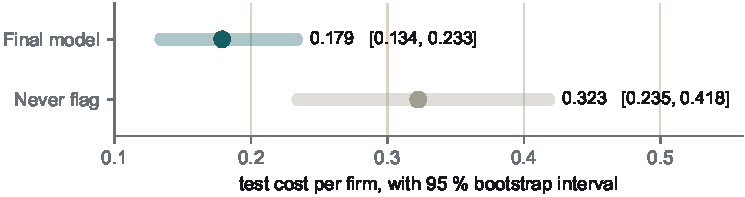
\includegraphics{bootstrap.pdf}\par\vspace{2mm}\raggedright
  \begin{columns}[T,onlytextwidth]
    \column{0.47\textwidth}
      \aside{Hoeffding (Lecture 2): too wide to decide}\par\vspace{1mm}
      $\pm\, C_{FN}\sqrt{\log(2/\alpha)\,/\,2m} \,=\, \pm\,0.37$
    \column{0.47\textwidth}
      \aside{Bootstrap, 1,000 resamples of the test firms:}\par\vspace{1mm}
      gain in $[0.065,\; 0.228]$ per firm
  \end{columns}\par\vspace{3mm}
  \takeaway{The interval excludes 0: the model really beats not screening.}
\end{frame}

\begin{frame}{What if the costs were different?}
  \vspace{1mm}
  \begin{columns}[c,onlytextwidth]
    \column{0.66\textwidth}\centering
      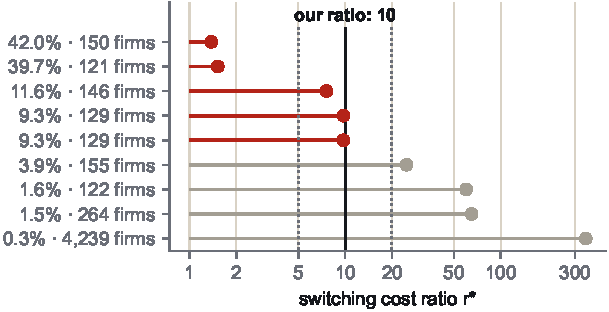
\includegraphics[width=\linewidth]{switching.pdf}
    \column{0.30\textwidth}
      A leaf is flagged once the cost ratio exceeds\par\vspace{2mm}
      \keyformula{$\displaystyle r^* = \frac{1-\hat\eta}{\hat\eta}$}\par\vspace{4mm}
      \aside{Any ratio between 9.75 and 24.8 gives the same decisions.}\par\vspace{3mm}
      \takeaway{Two leaves sit right at the edge.}
  \end{columns}
\end{frame}

\setkicker{RECOMMENDATION}
\begin{frame}{Our recommendation}
  \vspace{4mm}
  \begin{columns}[T,onlytextwidth]
    \column{0.47\textwidth}
      \actioncard[60mm]{risk}{1 \quad Action}{Flag every firm whose leaf has a bankruptcy share of at least 1/11: 8 ratios, a depth-4 tree.}\par\vspace{2.5mm}
      \actioncard[60mm]{ink}{2 \quad Assumptions}{A missed bankruptcy costs 10 false alarms; leaf shares are taken as probabilities.}
    \column{0.47\textwidth}
      \actioncard[60mm]{model}{3 \quad Versus no screening}{0.179 vs 0.323 per firm: 32 of 44 bankruptcies caught for 124 false alarms.}\par\vspace{2.5mm}
      \actioncard[60mm]{bench}{4 \quad What would change it}{A cost ratio below 9.75 unflags two leaves; below 7.6, a third.}
  \end{columns}
\end{frame}

\setkicker{LIMITATIONS}
\begin{frame}{What to keep in mind}
  \vspace{4mm}
  \begin{columns}[T,onlytextwidth]
    \column{0.47\textwidth}
      \begin{points}
        \item \textbf{Assumed costs.} The 10 : 1 ratio is stipulated.
        \item \textbf{No time dimension.} A random split, not a forecast of future years.
        \item \textbf{Repeated firms?} The same firm may appear in several years.
      \end{points}
    \column{0.47\textwidth}
      \begin{points}
        \item \textbf{Few bankruptcies.} 176 in training, 44 in the test set.
        \item \textbf{Fragile leaves.} Two leaves sit 0.002 above the threshold, within noise ($\pm 0.026$).
        \item \textbf{Unstable shortlist.} A 7-ratio selection works about as well.
      \end{points}
  \end{columns}
\end{frame}

% =====================================================================
%  CLOSING
% =====================================================================
{\setbeamercolor{background canvas}{bg=ink}\setbeamertemplate{background}{}
\begin{frame}[plain]
  \begin{tikzpicture}[remember picture, overlay]
    \node[anchor=north west, inner sep=0, text width=70mm, align=left] at ([xshift=10mm, yshift=-14mm]current page.north west)
      {{\color{risk}\caps{THANK YOU}}\\[5mm]
       {\display\fontsize{38}{42}\selectfont\color{paper}Questions?}};
    \node[anchor=north west, inner sep=0, text width=60mm, align=left, text=paper] at ([xshift=-70mm, yshift=-15mm]current page.north east)
      {{\color{paper!55!ink}\caps{THREE TAKEAWAYS}}\\[4mm]
       {\color{risk}\rule[0.33ex]{1.2em}{1.1pt}}\; \textbf{Costs, not accuracy}: flag when $P \ge 1/11$.\\[3mm]
       {\color{risk}\rule[0.33ex]{1.2em}{1.1pt}}\; \textbf{LASSO + a small tree}: 45\,\% lower cost on unseen firms, with readable rules.\\[3mm]
       {\color{risk}\rule[0.33ex]{1.2em}{1.1pt}}\; \textbf{A forest} is about 10\,\% cheaper: the price of interpretability.};
    \node[anchor=south west, inner sep=0, align=left] at ([xshift=10mm, yshift=9mm]current page.south west)
      {{\ttfamily\scriptsize\color{paper!75!ink}github.com/yassineerraji/Augmented-Decision-Final-Project}\\[2.5mm]
       {\color{paper!55!ink}\caps{YASSINE ERRAJI \enspace·\enspace WILLIAM PELTIER \enspace·\enspace BEN DAESH \enspace·\enspace SIMON AMAR}}};
  \end{tikzpicture}
\end{frame}}

\end{document}
